% Introduction :

\section{Introduction}

% Why did we do the work?
% What were the central motivations and hypotheses?
% The objectives of the work?
% What will this work show the reader?
% Why is it important?
% What should the reader watch for in the paper?
% What are the interesting high points?
% What strategy did we use?
% What should the reader expect as conclusion?

In order to characterize performance metrics, nuclear fuel cycle analysis 
requires calculation and optimization of myriad physical, nuclear, chemical, 
industrial, and political phenomena. Furthermore, complex systems such as 
nuclear process physics, facility deployment, and material routing each each 
must be modeled simultaneously for even the simplest of nuclear fuel cycle 
simulations. 

% MJG - I'm hesitant about using the phrase 'full detail'. I think we can be
% more precise.

Historically, nuclear fuel cycle simulators have addressed this with software 
ranging from spreadsheet driven flow calculators to full detail industrial 
models. To date, current tools are either static, fleet-based, or 
privately distributed. An alternative to these approaches is a dynamic, 
agent-based simulator with an open platform. 

Modern insight indicates that dynamic nuclear fuel cycle analysis more 
realistically supports a broader range of simulation goals than static analysis 
\cite{piet_dynamic_2011}. Similarly, experience in the greater field of systems 
analysis indicates that agent-based modeling enables more flexible simulation 
control, without loss of generality \cite{thatpapermattsent}. Finally, 
openness allows cross-institutional collaboration, increases code robustness, 
and enables the cultivation of an ecosystem of calculation options, 
\cite{softwarecarpentryresource}.  

Myriad challenges in nuclear fuel cycle analysis could be 
addressed with an agent-based framework for simulation and tracking of 
transformation and trade of resources between facilities within institutions 
and regions.  

\subsection{Background}

% Who else has done what?
% How did they do that?
% What did we do before this?
% What is new?

% Common goals of fuel cycle simulation/simulators (driving r&d focus,
% approximating tech. impacts, etc.)
% Previous work (cite all the tools!)
% Limitations of previous simulators by others (fleet-based, closed
% development, inflexible infrastructure)
% Previous attempts by this group (GENIUS v1/v2)
% note NGFCS

Simulators drive \gls{RDD} by calculating metrics that can be compared among fuel 
cycles. Examples include measures of economic feasibility (i.e., \gls{LCOE}), 
proliferation risk (i.e., total separated Pu), and environmental performance 
(i.e., waste volume). 

Methods for calculating those metrics vary among simulators. Some model the fuel cycle at static equillibrium, while others 
capture fuel cycle dynamics.  Similarly, while some simulators discretely model 
material and and facilities, others track streams of materials and 
fleets of facilities in an aggregated fashion. Depending on their intended use, 
simulators often model some aspect of the fuel cycle in great detail. For this 
reason, simulators specialize in economics, material isotopics, or 
transmutation detail, where others do not. 

Historically, the national laboratories have driven development and regulated 
the use of their own tools such as \gls{VISION}\cite{jacobson_verifiable_2010}, 
\gls{DANESS}\cite{van_den_durpel_daness_2009}, 
\gls{DYMOND}\cite{modeling_yacout_2005}, and 
\gls{NFCSim}\cite{schneider_nfcsim:_2005}, while universities and industry have 
simultaneously developed tools of their own as well, such as 
\gls{CAFCA}\cite{guerin_benchmark_2006}.

The \Cyclus code arose out of the 
\gls{GENIUSv2}\cite{oliver_studying_2009,huff_geniusv2_2009} code. That software 
itself was the result of lessons-learned from an \gls{LDRD} project at 
\gls{INL}, 
\gls{GENIUSv1}\cite{dunzik-gougar_global_2007,jain_transitioning_2006} which 
captured regional behaviors in fuel cycle scenarios. 


\subsection{Motivation}
% Gently reiterate the above need. 
% There should be a hero narrative here
% There was a gap in the capabilities of simulators.
% \Cyclus, a hero, came in to fill that gap. 

% MJG - @gonuke has always cited method-to-method comparisons as the primary
% benefit \Cyclus can bring to the table. Do we want to frame the hero narrative
% in that context? The more I think about, the more I feel like this is a
% secondary argument. I'll take a crack at a few sentences below.

In addition to providing the fundamental features expected in fuel cycle 
simulators, the \Cyclus paradigm enables two major capabilites that previous 
simulators were lacking. First, it enables simulations at multiple levels of 
fidelity. Second, it facilitates direct comparison of modeling methodologies.

% MJG - I don't claim that all of this belongs in the beginning of this
% subsection, but here's some more content. 

Modeling the evolution of a physics-dependent, international nuclear fuel supply
chain is a difficult problem. To date, it has been treated relatively
lightly. Tools have either focused on macro effects, e.g., the fleet-level
stocks and flows of commodities, or micro effects, e.g., the used fuel
composition fast reactor fuel. Accordingly, each focus has driven the
development of these tools, rendering the task of answering questions between
the macro and micro levels either impossible or difficult and time consuming. 

\Cyclus separates the problem of modeling a
physics-dependent supply chain into a simulation kernel and archetypes that
interact with the kernel during a simulation. The kernel is responsible for the
deployment and interaction logic of entities in the simulation. Physics
calculations are constrained to individual archetypes. Accordingly, specialists
in a given field can utilize their time and resources in modeling a specific
process associated with the nuclear fuel cycle, e.g. reprocessing and advance
fuel fabrication, rather than also modeling the entirety of the cycle.

% we could use a specific example of Cosi's equivalence method below
Because \Cyclus uses a modular archetype approach, comparing two archetypes is
straightforward. Consider a case in which an analyst would like to compare the
effect of using different models to determining input fuel composition for fast
reactors. A variety fuel fabrication archetypes can be developed and used
interchangably to analyze the effect of each on a simulation's output.

\subsubsection{Modular Architecture}
% Motivation for encapsulated plug-in architecture 
% enables ecosystem, ease of contribution across institutions
% enables myriad levels of simulation fidelity
% enables FC analyses that can compare ‘apples to apples'

Draw from and cite the ``Open Architecture and Modular Paradigm'' ANS summary.

We expect that there are a number of types of users and developers who will 
interact with the \Cyclus framework. Those people fall into a number of 
categories. All such people benefit from the modular architecture. 

\begin{figure}[htbp!]
\begin{center}
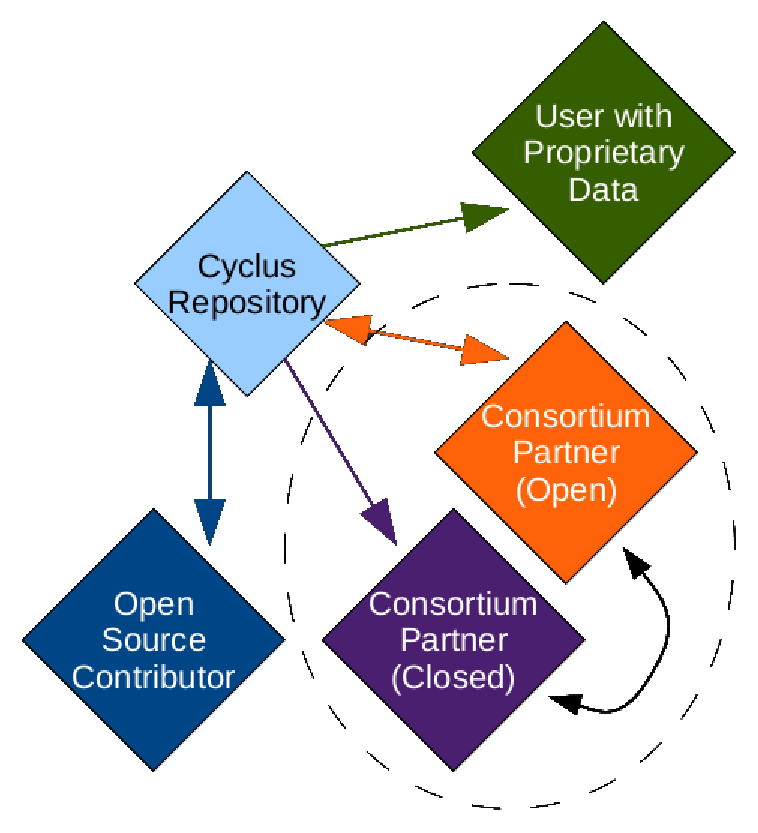
\includegraphics{./images/modifiedopen.eps}
\end{center}
\caption{The \Cyclus framework enables fully open, partially open, and fully 
closed collaborations.}
\label{fig:modifiedopen}
\end{figure}

\subsubsection{Agent-based Paradigm}
% superior detail in capturing simulation dynamics
% more flexible control over behavior
% describe Region/Institution/Facility hierarchy
% note importance of generic resource exchange paradigm

ABM is modern, sophisticated, true to reality, and it takes advantage of modern
computing resources. Furthermore, agent-based modeling provides an analyst a
more natural perspective from which to model a given problem. In the nuclear
fuel cycle context for example, an analyst can design an agent with
reactor-related logic and a separate agent with fuel fabrication-related logic.

System dynamics popular approach for modeling nuclear fuel cycles in current
tools (cite VISION/CAFCA). It has been shown in the literature
\cite{macal_agent-based_2010} that any system dynamics model can be translated
into an agent-based model. Furthermore, it has been shown that agent-based
techniques can provide a richer model than can system dynamics. Formally, the
set of system dynamics models is a strict subset of agent-based models.

\subsubsection{Discrete Resource Tracking}
% enables more realistic models and metrics
% material routing metrics
% shadow fuel cycles
% etc.

Not all simulations can be successfully run with a fleet-based model that 
doesn't distinguish between discrete materials. Shadow fuel cycles are an 
example. 

A discrete resource model allows for a range of modeling granularity. In the
macroscopic extreme, it is equivalent to time-stepped continuous flow. In the
microscopic extreme, the model is capable of representing individual fuel
assemblies.

